\chapter{Development Trade-offs and Learning Curve}

According to Stack Overflow’s 2024 Developer Survey, Rust remained the most admired programming language, with an admiration rate of 82.2\%, while C++ received an admiration score of 53.1\%. Rust also proved more desirable (28.7\% vs. 18.3\% for C++); however, when it comes to actual usage, C++ continues to lead. Among all respondents, 23\% reported working primarily with C++, compared to only 12.6\% for Rust. This trend is even more pronounced among professional developers—20.3\% use C++ versus 11.7\% for Rust—and among those learning to code, where 39.3\% prefer C++ over Rust’s 18.5\% \cite[]{Technology2024Stack}. 

These contrasting findings raise an important question: How can Rust be both more admired and desired, yet fall short of C++ in terms of professional and educational usage? Several factors may contribute to this discrepancy, including the relative age of the language, industry legacy, ease of use, and the availability of job opportunities.

\section{Advantages and Challenges of choosing Rust}
A study by K. R. Fulton and A. Chan examined the benefits and drawbacks of adopting Rust by conducting interviews with senior and professional software engineers from companies using—or attempting to adopt—Rust, as well as engaging with various online Rust communities. Participants in the study expressed strong support for Rust’s safety features, noting high confidence in its memory safety (90\%), concurrency safety (84\%), and absence of null pointers (81\%). Additionally, 87\% of respondents cited Rust’s performance as a key advantage.

The study also investigated challenges related to code migration and interoperability. Among participants who had ported code to Rust, 52\% found the process of porting existing C++ code to Rust to be somewhat or extremely easy. In contrast, only 43\% reported that interoperating with existing C++ code was somewhat easy. Furthermore, the study revealed that 59\% of participants considered Rust to be more difficult to learn than other languages, and 55\% stated that it takes longer to produce a compilable Rust program compared to other languages \cite[]{fultonBenefitsDrawbacksAdopting}.

\paragraph{}

An analysis of the 2024 State of Rust survey reveals key challenges faced by programmers when using or adopting Rust. Among respondents who do not use Rust, the most common reason cited—excluding those who indicated they simply "haven't gotten around to it" (70.5\%)—was the difficulty or time required to learn the language. Specifically, 30.6\% of respondents reported that Rust is either "too difficult to learn" or "takes too much time to learn," a figure that remains within the margin of error compared to the 2023 survey results \cite[]{2024StateRust}. These findings align with prior research by Fulton and Chan, who examined the benefits and drawbacks of adopting Rust and similarly identified learning difficulty as a key barrier to adoption \cite[]{fultonBenefitsDrawbacksAdopting}.

Additionally, 63.7\% of respondents indicated that they no longer use Rust but would like to in the future if the opportunity arises. Meanwhile, 36.0\% of respondents cited external factors, such as changing goals and requirements in their professional use of Rust, as the reason for no longer using it. This marks a decrease from 45.7\% in 2023, possibly indicating that Rust is becoming more integrated into professional development settings.

This trend is further supported by the continuous increase in daily or near-daily Rust usage, which grew from 47.3\% in 2022 to 49.3\% in 2023 and 53.4\% in 2024. Similarly, the percentage of participants who claim proficiency in writing production-ready Rust code has risen from 42.3\% in 2022 to 47.0\% in 2023, reaching 53.5\% in 2024. This suggests a growing number of proficient Rust developers producing usable code.

The proportion of developers using Rust for the majority of their coding tasks has increased from 29.8\% in 2022 to 33.9a\% in 2023 and 38.2\% in 2024, indicating a rising adoption of Rust in professional settings. This is further reinforced by the increase in organizations making non-trivial use of Rust, from 35.4\% in 2022 to 38.7\% in 2023 and 45.5\% in 2024.

In 2024, respondents working in professional settings cited several key reasons for using Rust: developing relatively correct and bug‐free software (87.1\%), its strong performance (84.5\%), its focus on security and safety (74.8\%), and the overall enjoyability of programming in Rust (71.2\%). Moreover, 82.1\% of respondents stated that "using Rust has helped us achieve our goals," and 77.9\% indicated they would choose Rust again in the future \cite{2024StateRust}.

\section{Comparing Development Tooling}
We wish to compare the development of software in Rust vs. C++ by looking at the tooling available for either language. C++ has a matured toolchain developed over many decades, with Rust toolchain lacking behind C++'s. 

\section{Comparing Merge Request Times in Rust and C++}
To compare the development experience between Rust and C++, we analyze the average time taken for a pull request (PR) to be merged into its respective repository. The average PR merge time serves as the primary metric for comparison, allowing us to gauge efficiency in handling contributions to projects.

We utilize GitHub’s publicly available API to retrieve the top 100 repositories for Rust and C++, sorted by the number of GitHub stars received. These stars provide a good metric on the popularity of the repository. The API is used to extract various repository metrics, including the timestamps for PR creation and merge events, as well as the number of contributors involved in each repository. By accounting for the number of contributors, we aim to compare similarly sized projects rather than projects with vastly different levels of activity.

To facilitate a fair comparison, repositories are grouped based on the number of contributors, enabling us to analyze PR merge times within similarly sized projects. To achieve this, we define bins for categorizing repositories according to contributor count:

Each repository is assigned to an appropriate bin based on its number of contributors. Within each bin, we compute the median of the average PR merge times of all repositories in that bin. This binned median merge time is then used for visualization and comparison between Rust and C++ repositories. By organizing data in this manner, we can discern patterns and trends in PR merge efficiency across different project sizes.

To visually represent the collected data, we use scatter plots where each point corresponds to a repository, and its coordinates denote the number of contributors and the median PR merge time. Additionally, we plot the average of all computed binned median merge times onto the graph to provide a clearer comparative trend between Rust and C++. This approach allows for an intuitive interpretation of how the two languages differ in terms of development workflow and contribution processing.

To further contextualize our findings, we apply the same methodology to 100 repositories from 3 other widely used programming languages, including Python, Java, and JavaScript. By expanding the analysis beyond Rust and C++, we can place our results within a broader spectrum of development experiences and identify whether the observed trends are unique to Rust and C++ or are part of a more general pattern across languages.

By analyzing the distribution of PR merge times across projects of varying sizes, we gain insight into how Rust and C++ differ in terms of developer efficiency and workflow. The results provide a data-driven perspective on contribution processing in these languages, which may help inform developers' choices when selecting a language for software development.

\begin{figure}
    \centering
    \subfloat[\centering label 1]{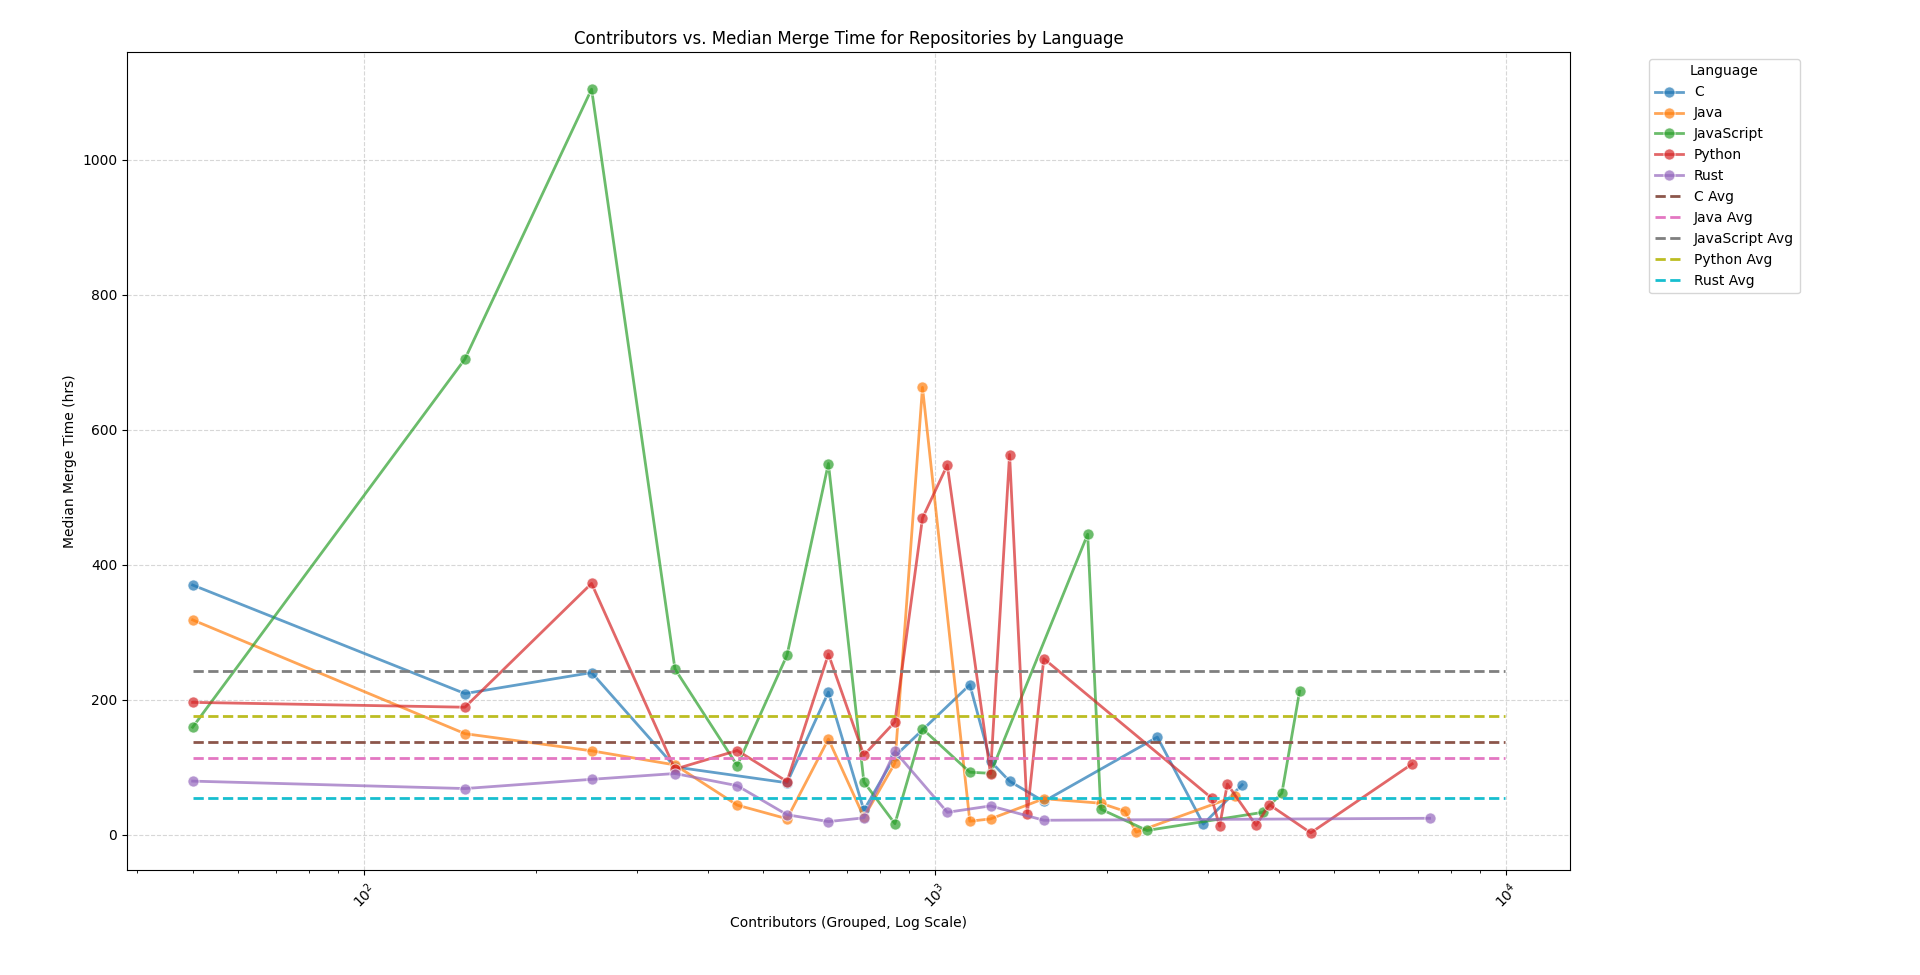
\includegraphics[width=0.45\textwidth]{images/graph1.png}}
    \hspace{0.5cm} % Adds some space between the figures
    \subfloat[\centering label 2]{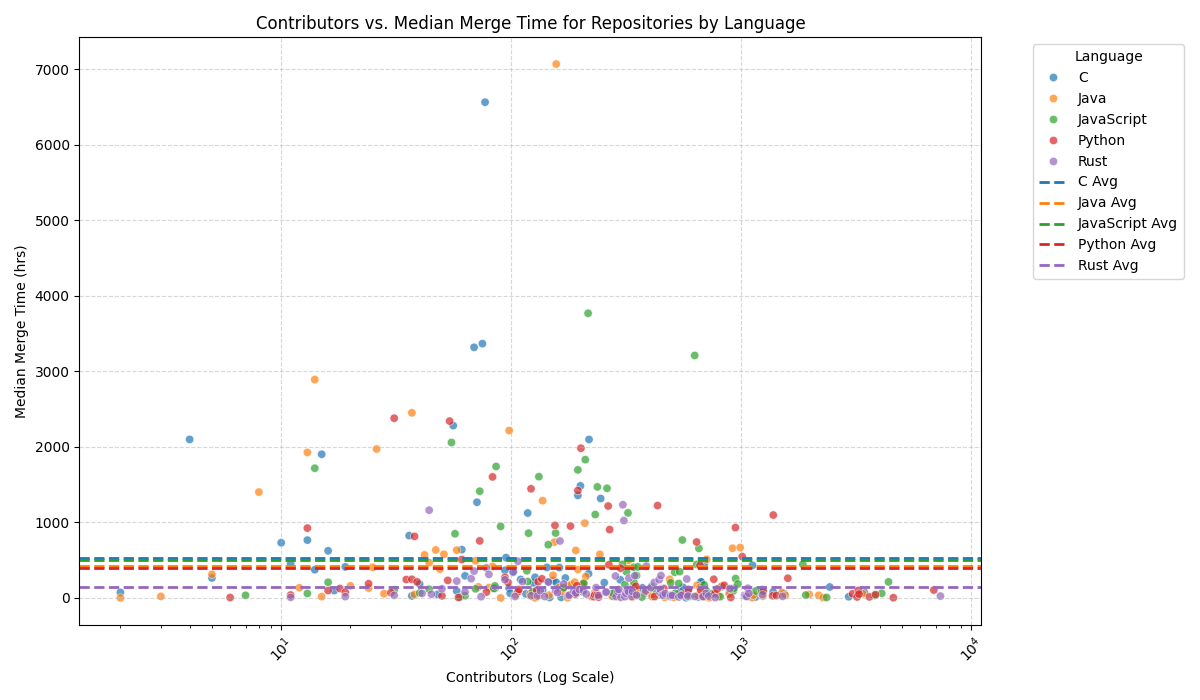
\includegraphics[width=0.45\textwidth]{images/graph2.png}}
    \caption{2 Figures side by side}%
    \label{fig:example}%
\end{figure}


% \begin{figure}[htbp]
%     \centering
%     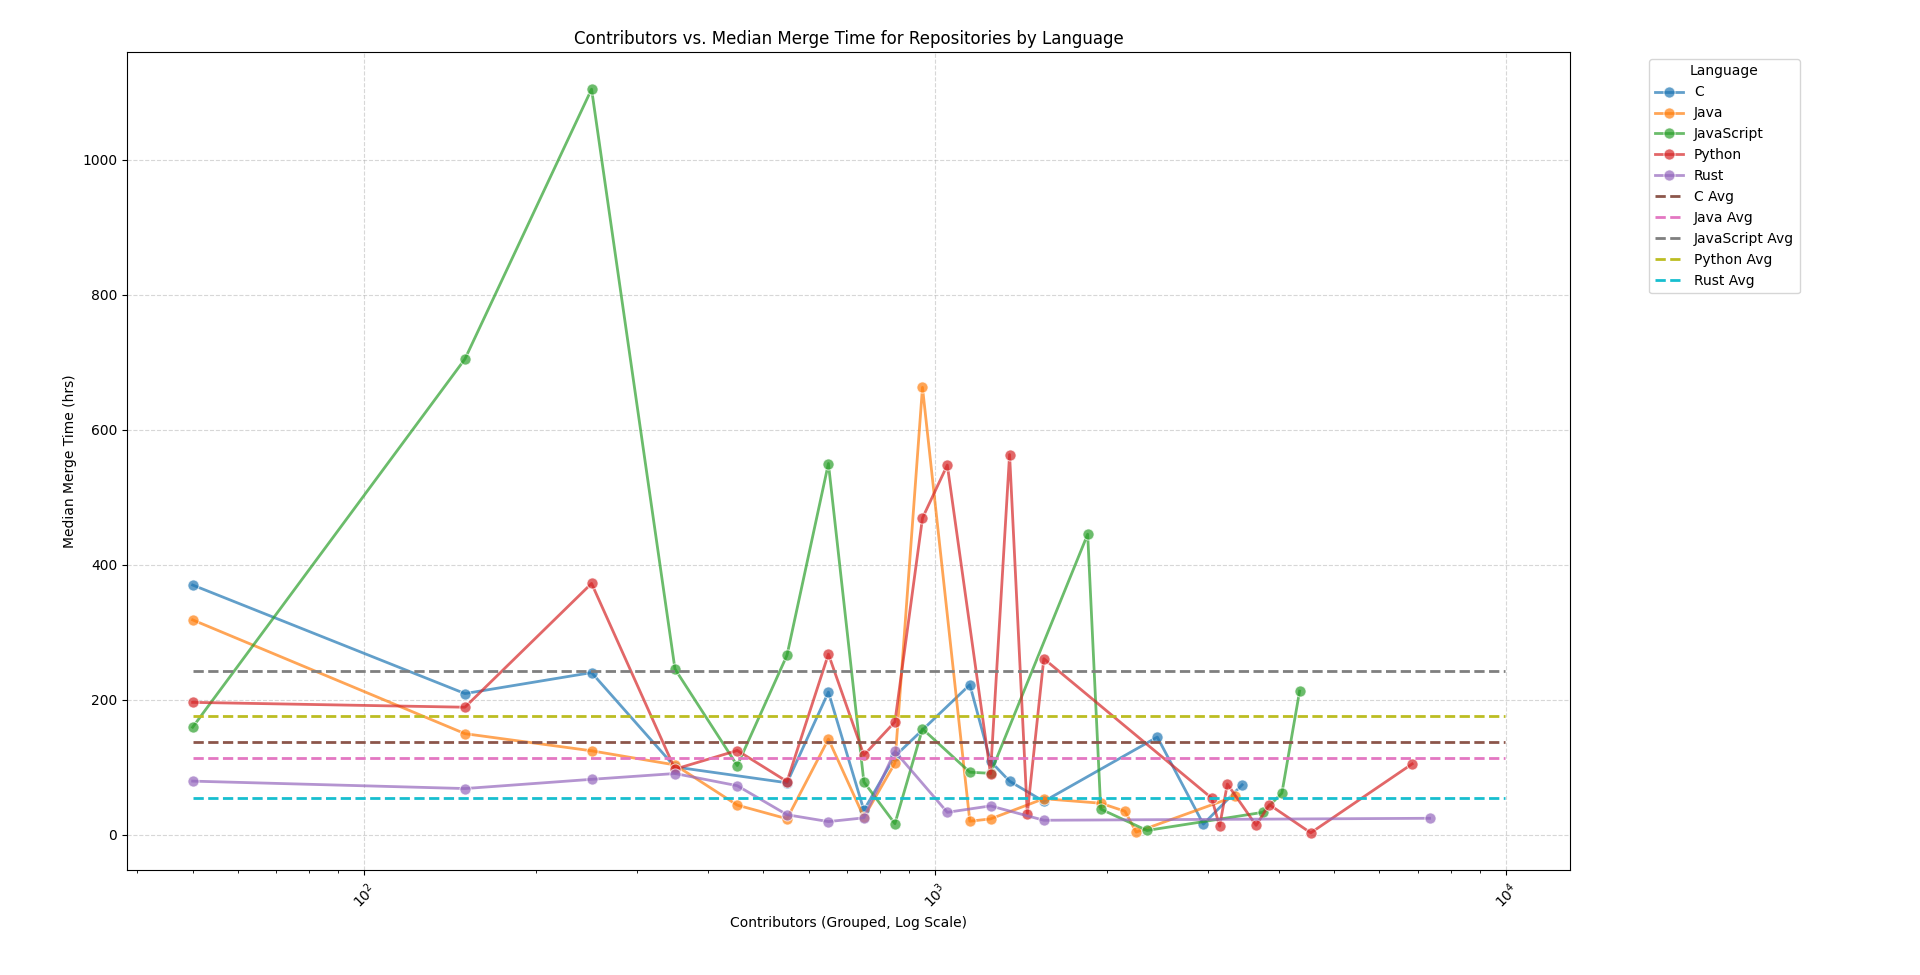
\includegraphics[width=0.8\textwidth]{images/graph1.png}
%     \caption{Descriptive caption explaining the figure.}
%     \label{fig:example1}
% \end{figure}
% \begin{figure}[htbp]
%     \centering
%     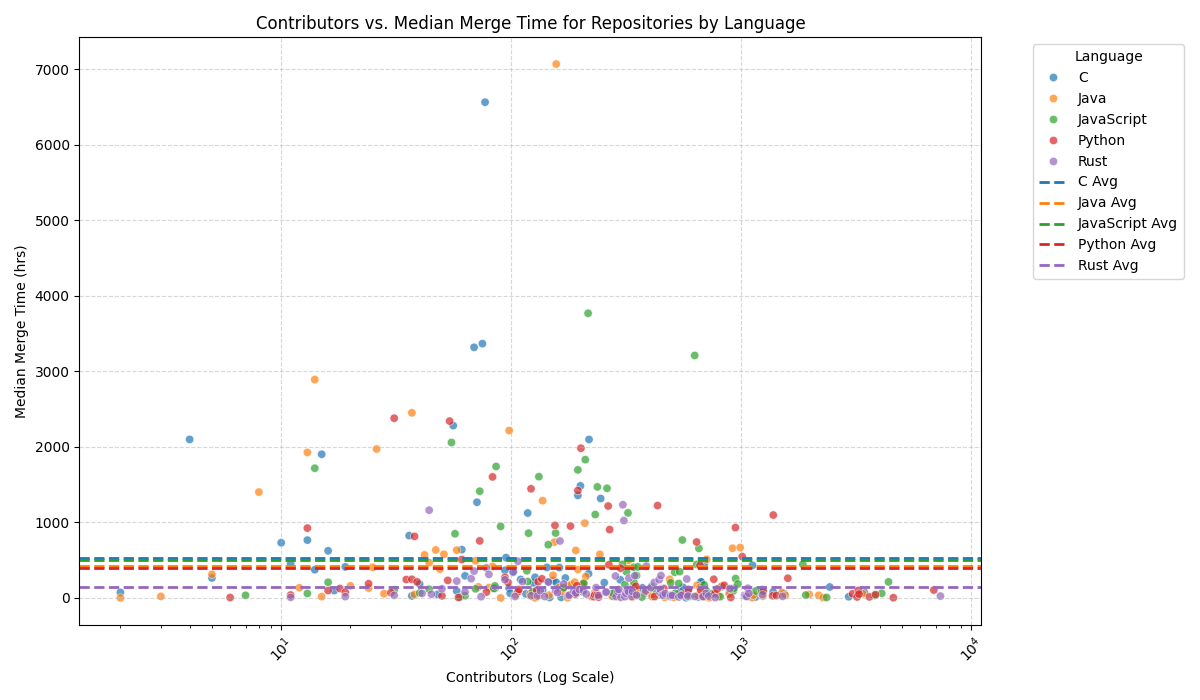
\includegraphics[width=0.8\textwidth]{images/graph2.png}
%     \caption{Descriptive caption explaining the figure.}
%     \label{fig:example2}
% \end{figure}

A comparative analysis of merge times between C++ and Rust was conducted across 149 Rust repositories and 148 C++ repositories. The results indicate that the average merge time for Rust is 159.98 hours, whereas for C++, it is significantly higher at 404.83 hours. The standard deviation for Rust is 235.15 hours, while for C++, it is 761.84 hours, suggesting greater variability in merge times for C++.

Examining quartile-based statistics, the first quartile (25th percentile) for Rust exhibits a merge time of 26.65 hours, whereas C++ demonstrates a substantially higher value of 64.40 hours. This represents a 241\% increase in merge time for C++ relative to Rust. Similarly, at the 50th percentile (median), Rust achieves a merge time of 77.53 hours, while C++ requires 130.23 hours, reflecting a 168\% longer merge time for C++. These findings suggest that Rust exhibits consistently faster and less variable merge times compared to C++.